\chapter{Literature Review}

This chapter aims to critically analyze the existing literature and related work on cloud computing and OpenID Connect (OIDC) protocols, focusing on identifying security risks and highlighting gaps in current research. The chapter will provide a foundation for understanding the complexities and challenges of securing cloud applications using OIDC by examining these areas. It will also offer an overview of cloud computing and OIDC to contextualize their interrelated roles in modern technology environments.

\section{Overview of Cloud Computing}
Cloud computing is a service model that provides on-demand access to a wide range of computing resources via the internet, including servers, storage, databases, networking, software, and analytics \citep{rashid2019cloud}. These services are designed to be easily manageable and deployable, often requiring minimal effort from the user. For example, users can quickly launch servers using a web browser through Cloud Service Providers (CSPs) such as AWS, Google Cloud and Microsoft Azure. 

Beyond simply running applications, cloud computing is evolving with new concepts like mobile cloud computing. One such concept is mobile cloud computing (MCC), a popular architectural model that integrates cloud computing with mobile technology. This model allows mobile devices to leverage the extra power and storage capacity of cloud-based resources, helping to overcome mobile hardware limitations \citep{mcc}. However, such models pose challenges to latency, data security, and network dependency. Addressing these issues requires robust network infrastructure, efficient data encryption, and effective management strategies to ensure privacy and reliability.

\section{Deployment Models}
The cloud offers different deployment models, each with varying levels of complexity and control, allowing consumers to choose the best fit for their needs, typically classified into public, private, hybrid, and community clouds. Security is a critical aspect that influences the choice of a deployment model; see Table \ref{table:cloud_comp} for a comparison. 
\begin{itemize}
    \item  \textbf{Public Cloud} - This model is the most used method to deploy applications in the cloud, preferred for running web applications, file sharing, and non-critical systems needed top-level privacy \citep{cloudmodel}. Public cloud services are also considered more cost-effective as the consumers can pay as they go. Public cloud providers often have multiple data centres worldwide, offering redundancy and high availability. This ensures that services remain available even if one data centre experiences issues. Public cloud providers also offer a range of managed services, such as databases, machine learning tools, and analytics platforms, which allow organizations to leverage advanced technologies without maintaining the underlying infrastructure. 
    
    While public clouds offer numerous benefits, security remains a primary concern. Key security considerations include data privacy and ensuring that sensitive data is encrypted and managed securely. Organizations must also ensure that their use of the public cloud complies with industry regulations and standards. Properly managing access controls and user permissions is essential to protect resources. Businesses should also consider strategies to avoid vendor lock-in to maintain flexibility and control  \citep{cloudmodel}.
    
    \item  \textbf{Private Cloud} - A Private cloud is a deployment model dedicated to a single consumer who does not share resources with multiple users to maintain a high level of privacy. The organization manages its resources and who has access to it. Some private clouds are also hosted in a local data centre to have greater infrastructure separation \citep{cloudmodel}. The principal characteristic of this model is to provide exclusive access to the resources only to the organisation, ensuring more significant levels of privacy and security. 
    
    However, the greater flexibility to customize the private cloud environment to meet specific business needs and performance comes with its challenges. Building and maintaining a private cloud can be more expensive than public cloud services due to the need for dedicated hardware and skilled IT staff. Managing a private cloud environment requires expertise and can be complex, particularly for organizations with limited IT resources. Additionally, private clouds may have limitations in scalability, depending on the organization's infrastructure and resources \citep{private_cloud}. \newline
    \item  \textbf{Hybrid Cloud} - As the name suggests, the hybrid cloud model combines both public and private clouds to achieve the best of both worlds and create a flexible, scalable computing infrastructure with the desired amount of control for critical assets. This model allows organizations to leverage the benefits of both cloud types while addressing specific business needs related to security, performance, and cost efficiency. By integrating public and private clouds, organizations can dynamically manage workloads, optimize resource usage, and improve business agility \citep{cloudmodel}.

    While the hybrid cloud offers numerous advantages, it also presents particular challenges. Managing and integrating multiple cloud environments can be complex and require robust IT expertise and tools. Ensuring seamless connectivity and interoperability between public and private clouds is critical to achieving the desired benefits. Organizations must also address security and compliance issues across both environments, implementing consistent policies and procedures to protect data and maintain regulatory compliance that requires additional tools and expertise, increasing the costs for running such a model \citep{hybrid_model}.
   
    \item  \textbf{Community Cloud} - A community cloud is a cloud deployment model where several organizations share the infrastructure with common interests, goals, or regulatory requirements. This model is designed to meet the specific needs of a particular community, such as industry groups, government agencies, or academic institutions. The community cloud offers a balanced approach, combining the shared resource benefits of a public cloud with the enhanced security and compliance controls of a private cloud. Organizations within the community share the costs, making it a cost-effective solution \citep{cloudmodel}.
\end{itemize}

\begingroup
\centering
\setlength{\tabcolsep}{6.5pt} % Default value: 6pt
\begin{longtable}{|p{2cm}| p{3cm} |p{3cm} |p{3cm}|p{3cm}|}
\caption{Cloud Deployment model comparison}
    \label{table:cloud_comp}
\hline
\rowcolor{grey!15}
\textbf{Feature} & \textbf{Private Cloud} & \textbf{Public Cloud} & \textbf{Hybrid Cloud} & \textbf{Community Cloud} \\
\hline
\endfirsthead
\hline
\rowcolor{grey!15}
\textbf{Feature} & \textbf{Private Cloud} & \textbf{Public Cloud} & \textbf{Hybrid Cloud} & \textbf{Community Cloud} \\
\hline
\endhead
\hline
\endfoot
\hline
\endlastfoot

Cost & Higher initial investment; lower ongoing costs if managed well. & Typically lower initial investment; pay-as-you-go model. & Mix of both; can be cost-effective if managed properly. & Costs shared among organizations; generally lower than private cloud. \\
\hline
Security & High; dedicated infrastructure, more control. & Variable; depends on the provider’s security measures. & Variable; depends on integration and management. & Moderate; shared infrastructure with similar organizations. \\
\hline
Compliance & Easier to meet specific regulatory requirements due to dedicated resources. & May meet general compliance standards; might require additional controls for specific needs. & Can meet compliance if managed properly with both environments. & Often easier to meet compliance for shared needs of community members. \\
\hline
Scalability & Limited by physical resources and scaling can be expensive. & Highly scalable; can quickly adjust resources based on demand. & Highly scalable; combines public cloud's scalability with private cloud’s control. & Limited scalability; constrained by shared resources within the community. \\
\hline
Ownership & Owned and operated by the organization or a third party dedicated to the organization. & Owned and operated by the cloud service provider. & Ownership is shared between private and public components. & Owned and operated by the community or a third party dedicated to the community. \\
\hline
Use Cases & Suitable for sensitive data and mission-critical applications. & Ideal for general-purpose applications, web hosting, and businesses with variable needs. & Good for organizations needing a mix of private and public resources, such as data privacy and scalable resources. & Best for organizations with common interests or regulatory requirements, such as government agencies or academic institutions. \\
\hline
Control & High control over infrastructure and data. & Limited; control is restricted to what the provider offers. & Variable; control over private components is high but limited over public components. & Moderate; control is shared with other community members and governed by shared policies. \\
\hline
Reliability & High if well-managed. & High; providers offer redundancy and failover solutions. & High; combines the reliability of private and public cloud components. & Generally reliable; depends on the community's infrastructure and management. \\
\hline
\end{longtable}
\endgroup

\section{Risks}
\begin{itemize}
    \item \textbf{Access Control In the Cloud} - Access control in the cloud is critical to securing the system and sensitive data. However, managing the access control has risks, especially when the controls are misconfigured, as the cloud follows a shared responsibility for securing the systems between the customer and the cloud provider \citep{cloud_shared_resp}. Such misconfiguration of identity and access management (IAM) policies, weak authentication practices, and poor management for storing and rotating secret keys can lead to unauthorised access.  

    \item \textbf{Network Security } - Network security in cloud computing faces unique challenges that can compromise data and service integrity. One of the primary risks is insecure API endpoints, where attackers can exploit vulnerable APIs lacking proper authentication and encryption to gain unauthorized access to cloud resources, leading to data breaches and service disruption. Network security issues have a lot of commonalities with the traditional, like DDoS, Man-in-the-Middle (MitM)  and VM vulnerabilities, especially with cloud sharing infrastructure where the infrastructure is shared amongst many clients \citep{network_cloud}. If proper measures and configurations are not in place, attackers could move laterally across the cloud to infiltrate many systems and organisations simultaneously. 
    
    \item \textbf{Regulatory Compliance } - Cloud computing has added complexity as Cloud providers tend to be multi-regional, which presents significant challenges to organisations operating across different regions, and the areas are subject to strict requirements for data protection, security controls and data sovereignty. This risk, in particular, is not a security risk but rather a legal one, where not failure to comply with local laws and regulations such as HIPAA, GDPR, and PCI DSS could lead to financial and reputational damage \citep{legal_cloud_challenge}.
    
    \item \textbf{Malware on Mobile Cloud Computing } - Cloud computing has evolved from the traditional web application to being used for mobile, also known as Mobile Cloud Computing. Malware injection is a significant threat to MCC. Attackers can embed malicious code into legitimate mobile applications, leading to harmful activities such as stealing sensitive data or using cloud computing power for tasks like crypto mining, also known as cryptojacking \citep{cryptojacking}. The interconnected nature of cloud computing means that malware introduced into one device can potentially spread to other devices or services within the same cloud environment. For instance, if a cloud-based application becomes infected, all users accessing that application are at risk of having their data compromised. Once malware is injected, it can persistently attack the mobile device, extract valuable information, and send it back to the attacker, often without the user's knowledge.
    
    \item \textbf{Multi-tenancy} - Multi-tenancy security risks are very similar to the ones discussed in network security, as in a multi-tenant system, an organisation could use the same physical hardware as in a private deployment model. Such a system can lead to data leakages or unauthorised access if it is improperly configured or there are vulnerabilities in the cloud provider's software.   According to \citep{multi_tenancy_cloud_risk}, an attacker has a 40\% chance of allocating his VM besides the victims using tactics like side-channel attacks, which can be done with a moderate budget, making such attacks more probable.

\end{itemize}

\section{OpenID Connect Protocol}
OpenID Connect (OIDC) is a prevalent authentication layer based on the OAuth 2.0 protocol that provides a standardised way of authenticating and authorising users across web applications and apps \citep{oidc_intro}. OpenID Connect enables a secure sign-in experience and simplifies verifying user identities across various applications and platforms. This protocol allows applications to request and receive information about authenticated users from identity providers (IDPs), such as Google, Microsoft, and Facebook. The authentication process involves exchanging different types of tokens, usually in JSON Web Token (JWT) format, a widely adopted industry standard for exchanging information between two parties \citep{jwt}. These JWT tokens are then used as different kinds of Tokens, such as ID tokens, access tokens, and refresh tokens that contain claims or information about the user and the permissions they are allowed in the application and carry information about their sessions. Using these tokens, an application can authenticate and authorise users (Access Tokens), identify authenticated users (ID tokens) and provide a way to re-authenticate automatically without explicit login (Refresh tokens) \citep{oidc_tokens}; See Table \ref{table:oauth_terms} for more details. 

\begingroup
\centering
\setlength{\tabcolsep}{6.5pt} % Default value: 6pt)
\begin{longtable}{|p{4cm}|p{10cm}|}
\caption{OpenID Connect Terms}
    \label{table:oauth_terms}
\hline
\rowcolor{grey!15}
\textbf{Term} & \textbf{Description} \\ 
\hline

\textbf{Client} & The app that wants to access some data. \\ \hline
\textbf{Resource server} & The resource that the client wants to access. This is generally an API or an app that contains some data. \\ \hline
\textbf{Resource owner} & The data owner on the server. \\ \hline
\textbf{Authorisation server} & The main server which issues the tokens after successful authentication.\\ \hline
\textbf{Grant Type} & This is an authorisation given to the client to access the data on the resource server, which represents the specific permission the client is allowed to have. Grant types include Authorisation Code, Implict, and Client Credentials \citep{adv_api_sec}.  \\ \hline
\textbf{Access token} & The token issued by the authorization server to get the resources from the resource server. \\ \hline
\textbf{Refresh token} & A token that is used to retrieve a new access token after expiry. \\ \hline
\textbf{ID token} & A token that contains user identity information which can verify the identity of the user. \\ \hline
\end{longtable}
\endgroup

\subsection{Flows}
OpenID Connect provides a means to authenticate users and allow them to access data using different kinds of tokens. Still, in the real world, various requirements exist for diverse types of application architecture, such as mobile, server-server, and single-page applications. The OpenID Connect protocol is designed with multiple flows that try to balance security and usability to accommodate designs encompassing different security requirements and technical limitations. For example, some flows prioritise security by not exposing sensitive tokens on the user end. On the other hand, user experience is more of a focus, making it less secure. 
\par
In the coming section, we will discuss these critical flows to understand their advantages and disadvantages. Understanding the OpenID Connect flows and their characteristics allows one to choose the most appropriate method for their specific application scenario to balance security, functionality, and user experience.



\subsection{Implict Flow}
The Implicit flow is the most straightforward authentication flow in the OpenID Connect protocol. It is designed to accommodate client-side or single-paged applications (SPAs) running in a user's browser. This flow is primarily intended for scenarios where the client application cannot securely store client secrets, which are sensitive information for client authentication. This limitation is usually valid for web applications, mobile apps, and SPAs. This method directly issues tokens like ID Tokens, access tokens, and refresh tokens after the user successfully authenticates as part of the response without additional network requests (See Figure \ref{fig:implicit_flow} for the flow). Such an authentication process is advantageous as the resource access does not need many steps and reduces latency, as the tokens are available after user authentication. 

Despite the benefits of latency and simplicity, the Implicit Flow comes with particular security risks. The tokens are stored and handled directly in the client application or within the browser, making them vulnerable to various attacks. If the client applications are compromised and the tokens are exposed, this could lead to unauthorised access. The valuable tokens can be intercepted using different attacks, like man-in-the-middle attacks and cross-site Scripting, allowing the valid tokens to be replayed. The Implicit Flow provides quick and easy access to authentication tokens for client-side applications and has significant security challenges. It's crucial for developers to feel responsible and take proactive steps to apply appropriate security measures or, ideally, opt for more secure alternatives.
\begin{figure}[h!]
\centering
\caption{OIDC Implicit Flow}\label{fig:implicit_flow}
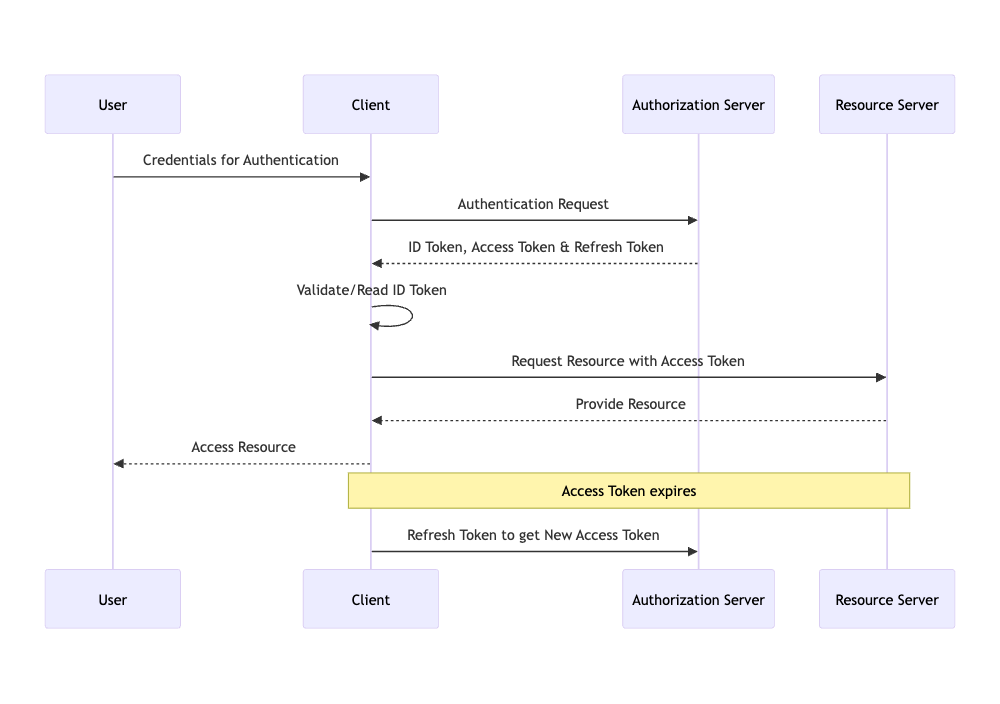
\includegraphics[width=\textwidth, height=320px]{pics/implicit_flow.png}
\end{figure}

\subsection{Authorisation Code Flow}
The Authorisation Code flow is another commonly used OpenID Connect flow that clients can use to verify the user's identity. This flow is crafted for applications such as server-to-server communication, which can store secrets, which are then used with the authorisation code, and handle the tokens without exposing them to the user. This method is one of the popular ways to implement OpenID Connect, as it provides a good balance between security and user experience and ensures a robust mechanism for authentication and authorisation. Figure \ref{fig:authorisation_flow} depicts the process of authorisation code flow, where a user tries to gain access to the resource after authentication. In contrast to the implicit flow, we can see that an authorisation code with a redirect URL is returned after authentication rather than tokens to the user. Combined with the correct client secret, this code returns the tokens only to the client and not the User. 

Given the benefits of this flow, this design is still not without potential risks, namely misconfigured URLs, which could let the attacker manipulate the redirect to a malicious site, Cross-Site Request Forgery (CSRF) if the tokens are not appropriately secured, the attacker can trick the user into submitting unintended requests, and also man-in-the-middle attacks, if the users authorisation code is intercepted and also the client secret is know due to other vulnerabilities then the attacker can impersonate as a legitimate user.

\begin{figure}[h!]
\centering
\caption{Authorisation Code Flow}\label{fig:authorisation_flow}
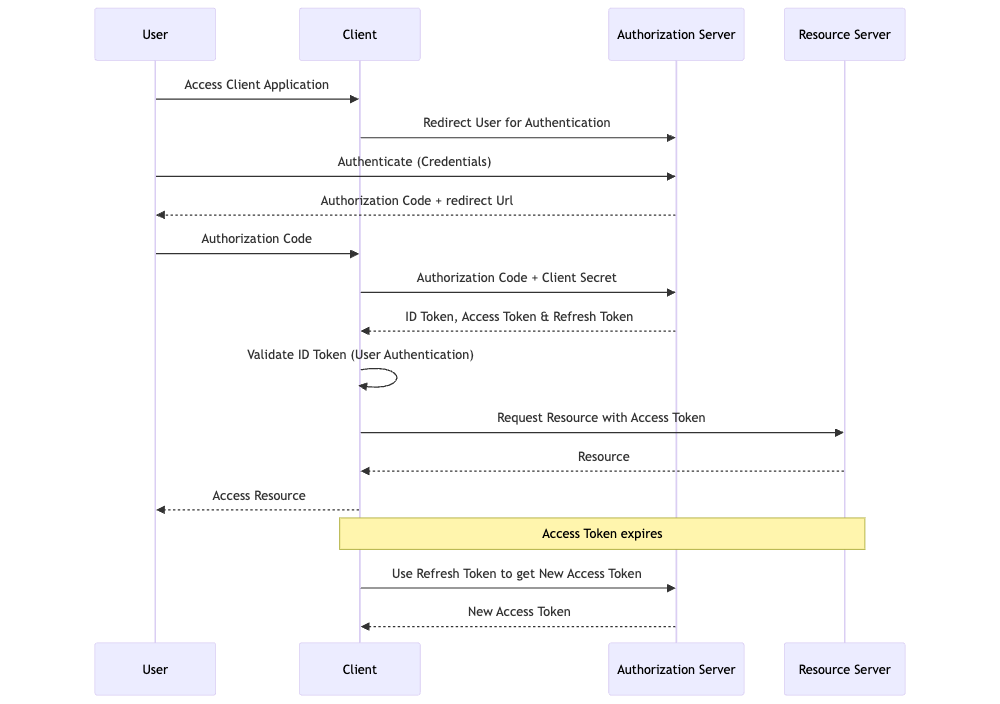
\includegraphics[width=\textwidth, height=320px]{pics/authorisation_flow.png}
\end{figure}

\newpage
\subsection{PKCE flow}
\label{sec:pkce_flow}
Proof Key for Code Exchange (PKCE) flow is an improvement to the authorisation code flow designed to harden the authentication process for public clients by protecting against several attacks, such as code interception \citep{pkce}. PKCE was introduced to address the vulnerabilities in clients, such as mobile and single-page applications (SPAs) that cannot store a client secret securely. In the authorisation flow, if the attacker intercepts the authorisation code and gets hold of the client secret with some known vulnerability, one can exchange this information for valuable tokens, providing the attacker with unauthorised access. 


\begin{figure}[h!]
\centering
\caption{PKCE Code Flow}\label{fig:pkce_flow}
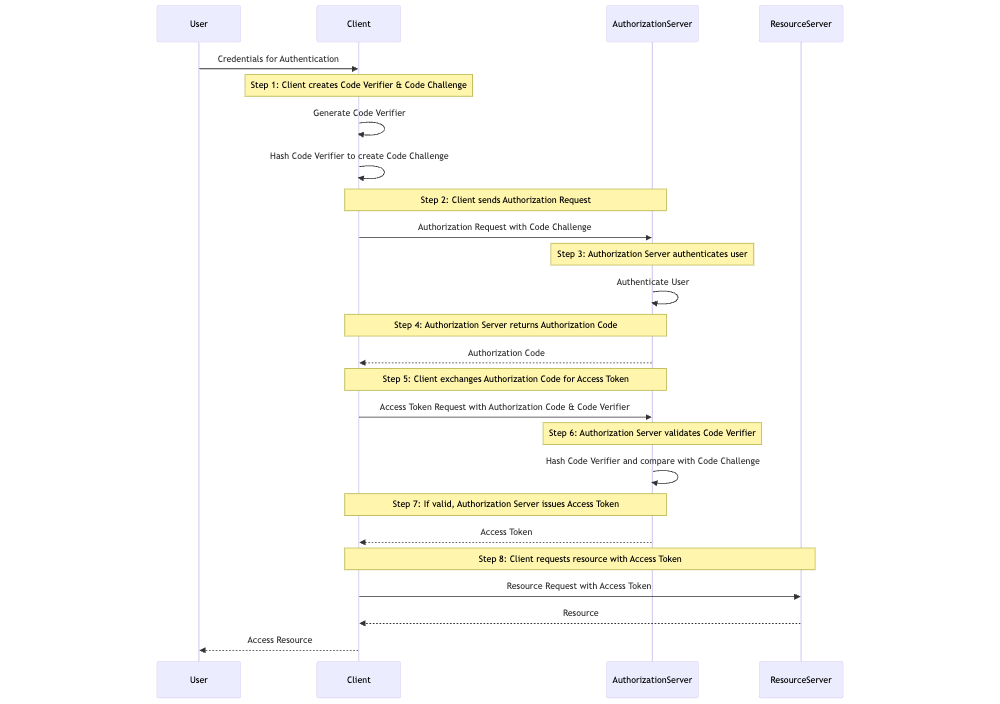
\includegraphics[width=\textwidth, height=320px]{pics/pkce.png}
\end{figure}

PKCE mitigates this risk by adding two additional steps: creating a "code verifier" and the "code challenge." When a client initiates the authorization request, it generates a random string called the "code verifier." This verifier is hashed using a secure method (such as SHA-256) to create the "code challenge" sent with the authorization request. The original code verifier must be provided when the client requests the access token. The authorization server hashes this verifier and compares it with the original code challenge. If they match, the server issues the access token (See Figure \ref{fig:pkce_flow}). This method ensures that the access token cannot be obtained without the authorisation code and the original code verifier. 

Like the other flows, PKCE also has potential risks, especially when the implementation of this method is not done correctly. The code verifier is an integral part of this process, and if the attacker can access it, it would make this flow vulnerable. The attackers have a few ways to obtain or even guess the code verifier. Since the code verifier has to be sent to the server and an insecure transmission is used, the code verifier can be intercepted. In addition, using random generators that are cryptographically secure can make the code guessable. On the one hand, the client has to implement all the steps correctly; on the other hand, the authorisation server also needs to validate the code, and if this is not done perfectly, then attackers could bypass PKCE.   


\begingroup
\centering
\setlength{\tabcolsep}{6.5pt} % Default value: 6pt)
\begin{longtable}{|>{\raggedright\arraybackslash}p{4cm}|>{\raggedright\arraybackslash}p{3.5cm}|>{\raggedright\arraybackslash}p{3.5cm}|>{\raggedright\arraybackslash}p{3.5cm}|}
    \caption{OpenID Connect Terms}
    \label{table:oauth_terms}
\hline
\rowcolor{grey!15}
\textbf{Feature} & \textbf{Implicit Flow} & \textbf{Authorization Code Flow} & \textbf{PKCE Flow} \\ \hline
\endfirsthead
\hline
\rowcolor{grey!15}
\textbf{Feature} & \textbf{Implicit Flow} & \textbf{Authorization Code Flow} & \textbf{PKCE Flow} 
\endhead
\hline
\endfoot
\hline
\endlastfoot

\textbf{Flow Type} & Direct token retrieval from the authorisation server. & Two-step process: The authorisation code is retrieved first and then exchanged for an access token. & It is the same as Authorisation Code Flow but adds a code verifier and code challenge for enhanced security. \\ \hline
\textbf{Security Level} & Lower security; tokens are exposed in URLs, making them vulnerable to interception. & More secure than Implicit Flow; tokens are kept server-side and retrieved via a back-channel. & Highest security; mitigates the risk of authorization code interception by adding PKCE parameters. \\ \hline
\textbf{Recommended For} & Single-page applications or Web applications that cannot store secrets securely. & Web and mobile applications with a secure backend. & Public clients, including SPAs and mobile apps, require enhanced security. \\ \hline
\textbf{Tokens Exposed in URL} & Yes, the access token is exposed in the URL fragment. & No, only the authorization code is in the URL and exchanged server-side. & No, only the authorization code is in the URL, with PKCE parameters providing additional security. \\ \hline
\textbf{Exchange of Authorization Code} & Not applicable; token is issued directly. & Yes, via a secure server-side request. & Yes, with the inclusion of a code verifier to ensure integrity. \\ \hline
\textbf{Vulnerability to Attacks} & Prone to interception attacks and token leakage. & Less vulnerable; however, the code could still be intercepted if not protected. & Minimizes risks, including code interception, through PKCE parameters. \\ \hline
\textbf{Token Storage} & Tokens are typically stored in browser storage, which may not be secure. & Tokens can be securely stored server-side. & Same as Authorization Code Flow; tokens are typically stored securely server-side. \\ \hline
\end{longtable}
\endgroup

\section{OIDC Security Risks}

The flows mentioned above are some industry-standard methods in OpenID Connect that carry out authentication and authorisation in different applications. While it shares some common vulnerabilities with other protocols, such as Man-in-the-Middle (MitM) attacks, Denial of Service (DoS), and Cross-Site Scripting (XSS), this section focuses on security risks that are particularly relevant to OpenID Connect. We will explore threats like Replay Attacks, Signature Manipulation, Malicious Endpoint Attacks, and PKCE Downgrade Attacks \citep{oidc_attacks}. 

\begin{itemize}
    \item \textbf{Replay Attacks} - Replay attack in OpenID Connect can be executed when an attacker successfully intercepts valid tokens like the authentication, refresh and ID tokens or gets hold of the authorisation code or code verifier. In this case of fraudulent access, the attacker could impersonate a user. However, OIDC has mechanisms to protect itself from such access; in particular, a claim called the nonce must be transmitted during request, and the client must check the nonce during each \citep{oidc_attacks}.
    
    \item \textbf{Signature Manipulation} - Signature manipulation attack targets the tokens in OIDC, namely the access token, refresh token and ID tokens. OIDC mandates that these JWT tokens are signed using a cryptographic algorithm like RS256 or a symmetric key algorithm like HS256 \citep{signed_token}. Using the signed tokens can prevent manipulating them to gain unauthorised access. \cite{oidc_attacks} mentions a case when an attacker can create tokens with a "none" algorithm, given the server handles it, allowing it to tamper the token. The tampered token would allow an attacker to commit identity spoofing and elevate their privilege to gain higher access, causing data loss and integrity risks.
    
    \item \textbf{Malicious Endpoint Attacks} - OpenID Connect is designed to operate using various endpoints that enable the crucial parts of authentication and authorisation processes. Table \citep{auth0_api_endpoints} presents some critical endpoints used in the context of OpenID Connect. The \textbf{/.well-known} is of interest to malicious attacks, as this endpoint is dynamic, which the clients use for the authentication process, containing vital configurations, namely supported scopes, endpoint, claims, jwks public key URL, authorisation endpoint, and Issuer \citep{oidc_attacks}. An attacker could tamper with the Discovery document to alter the endpoint URLs to redirect the client to a malicious server and gain unauthorised access. This attack can be achieved in two ways: tampering, where the discovery endpoint itself is tampered with, and poisoning the cache with malicious values. 

    % OIDC ENDPOINT TABLE BEGIN
    
    \begin{longtable}{|>{\raggedright\arraybackslash}p{4cm}|>{\raggedright\arraybackslash}p{11cm}|}
    \caption{OpenID Connect Endpoints}
    \label{table:outh_endpoints}
    \hline
    \rowcolor{grey!15}
    \textbf{OIDC Endpoint} & \textbf{Purpose} \\ \hline
    \endfirsthead
    \hline
    \rowcolor{grey!15}
    \textbf{OIDC Endpoint} & \textbf{Purpose} \\ \hline
    \endhead
    \hline 
    \endfoot
    \hline
    \endlastfoot
   \textbf{/authorize} & Initiates user authentication and authorisation. \\ \hline

    \textbf{/token} & Allows the access of tokens (access, refresh, and ID) in exchange for authorisation code or code_verify code.\\ \hline
    
    \textbf{/userinfo} & Retrieves profile information about the authenticated user. \\ \hline
    
    \textbf{/.well-known} & Provides crucial metadata for the OIDC identity provider, namely the locations of other endpoints and public keys used by the client to verify the signatures of tokens. This endpoint is dynamic, as the clients can use this metadata to get the latest public keys for token verification. \\ \hline
    
    \textbf{/revoke} & Allows the revocation of an access or a refresh token. \\ \hline

    \textbf{/introspect} & Allows to check the token information. \\ \hline
        
    \end{longtable}
    

    \item \textbf{PKCE Downgrade Attacks} - PKCE (See Section \ref{sec:pkce_flow}) is a flow developed to protect native applications from interception attacks \citep{pkce}. This flow adds several security layers or requests (See Figure \ref{fig:pkce_flow}) to achieve a secure authentication method for applications that cannot handle storing critical secret keys. Despite these measures, PKCE is still vulnerable to many attacks if no protection measures are taken. For example, in the PKCE Downgrade Attack, where the attacker tries to remove the \textbf{code\_challenge} and the authorising server does not validate it, the attack succeeds \citep{oidc_attacks}.

\end{itemize}


\section{Discussion}

While existing research provides valuable insights into the security of OIDC and Cloud applications separately, more studies need to be conducted specifically to address the security risks of OIDC in cloud environments. Cloud-based applications introduce unique challenges that are not fully covered by current research:

\begin{itemize}
    \item  \textbf{Multi-Tenancy Risks:} Cloud environments often host multiple tenants on shared infrastructure, increasing the risk of data leakage and unauthorised access between tenants.

    \item \textbf{Third-Party Integrations:} Cloud applications frequently integrate with numerous third-party services, amplifying the potential attack surface. Also, using External IDP providers like Auth0, which offers a managed OIDC connect user management service \citep{auth0-main}.

    \item \textbf{Configuration Management:} Misconfigurations in implementing OpenID connect with improper cloud access management could also cause unauthorised access and damage. Having an insight on what configurations on both sides the cloud configurations and OpenID Connect will help prevent certain attacks.

\end{itemize}

OpenID Connect plays a critical role in securing cloud-based applications, but the existing body of research needs to address the specific security challenges cloud environments pose. By focusing on the identified gaps and proposed areas for future research, the security of OIDC in cloud applications can be significantly enhanced. This will protect sensitive user data and bolster the trust and reliability of cloud-based services. This review does not focus on many other security risks and the mitigations that could be done in order to understand and prevent these risks. For a more comprehensive understanding, further reading is recommended (See Table \ref{table:further_reading}).

\begingroup
\centering
\setlength{\tabcolsep}{6.5pt} % Default value: 6pt)
\begin{longtable}{|>{\raggedright\arraybackslash}p{4cm}|>{\raggedright\arraybackslash}p{12cm}|>}
    \caption{Further Reading}
    \label{table:further_reading}
\hline
\rowcolor{grey!15}
\textbf{Author(s)} & \textbf{Title} \\ \hline
\endfirsthead
\hline
\rowcolor{grey!15}
\textbf{Author(s)} & \textbf{Title} \\ 
\endhead
\hline
\endfoot
\hline
\endlastfoot


% Begin the actual content
\cite{cloud_shared_resp} & \textit{Cloud computing security for multi-cloud service providers: Controls and techniques in our modern threat landscape} \\ \hline
\cite{Alouffi2021-yh} & \textit{A systematic literature review on cloud computing security:
               Threats and mitigation strategies}  \\ \hline
\cite{oidc_attacks} & \textit{Security Analysis of Real-Life OpenID Connect Implementations} \\ \hline
\cite{Mishra2019-uh} & \textit{Analysis of security issues in cloud environment} \\ \hline
\cite{openid_docs} & \textit{OpenID Official Documentation} \\ \hline
\cite{oidc_popular} & \textit{Best Current practices for Oauth/OIDC} \\ \hline
\cite{sec_privacy_cloud} & \textit{Security and privacy protection in cloud computing:
                  Discussions and challenges} \\ \hline
\cite{blockchain_oidc} & \textit{A novel secure and privacy-preserving model for {OpenID}
                  connect based on blockchain} \\ \hline

% Add more rows as needed

\end{longtable}



 



